
\documentclass[a4paper,12pt]{book}
\usepackage{tabularx}
\usepackage[a4paper, left=1in,right=1in,top=2cm,bottom=1.5cm]{geometry}
\usepackage{fancyhdr}
\pagestyle{plain}
\renewcommand{\chaptername}{Experiment}
\usepackage[utf8]{inputenc}
\usepackage{pdfrender}
\usepackage{xcolor}
\usepackage{ae}
\usepackage{multirow}
\usepackage{aecompl}
\usepackage{helvet}
\usepackage{afterpage}
\usepackage{graphicx}
\usepackage{caption}
\usepackage{array}
\makeatletter
\newcommand\@addfig{\relax}
\newcommand\addfig[1]{\global\long\def\@addfig{#1}}
\newcommand\@putfig{\@addfig\addfig{\relax}}
\newcommand\blankpage{%
	\null
	\vfill
	\@putfig%
	\vfill
	\thispagestyle{empty}% BEWARE, if you want the header and footer, you should put the correct style here
	\clearpage%
	\addtocounter{page}{-1}% BEWARE, if you want the left pages to be numbered, don't put this line, this is intended to have picture page with the same number as the facing text page
	\afterpage{\blankpage}}
	\makeatother

	\begin{document}
	%\pdfrender{StrokeColor=black,TextRenderingMode=2,LineWidth=0.1pt}
	\afterpage{\blankpage}
	\part{Hematology}

	\chapter*{\centering Compound Microscope}

	\begin{tabular}{p{5in} p{1in}}
		\textbf{Exp No:}  & \textbf{Date:}\\
	\end{tabular}
	\section*{Introduction}
	\par
	A microscope is an optical instrument which magnifies the image of an object.
	There are various types of microscope which use different types of lens and different principles of optics.
	Compound microscope is one of the most frequently used equipment in a medical laboratory.\newline

	\addfig{%
		\begin{figure}[h]
			\centering
			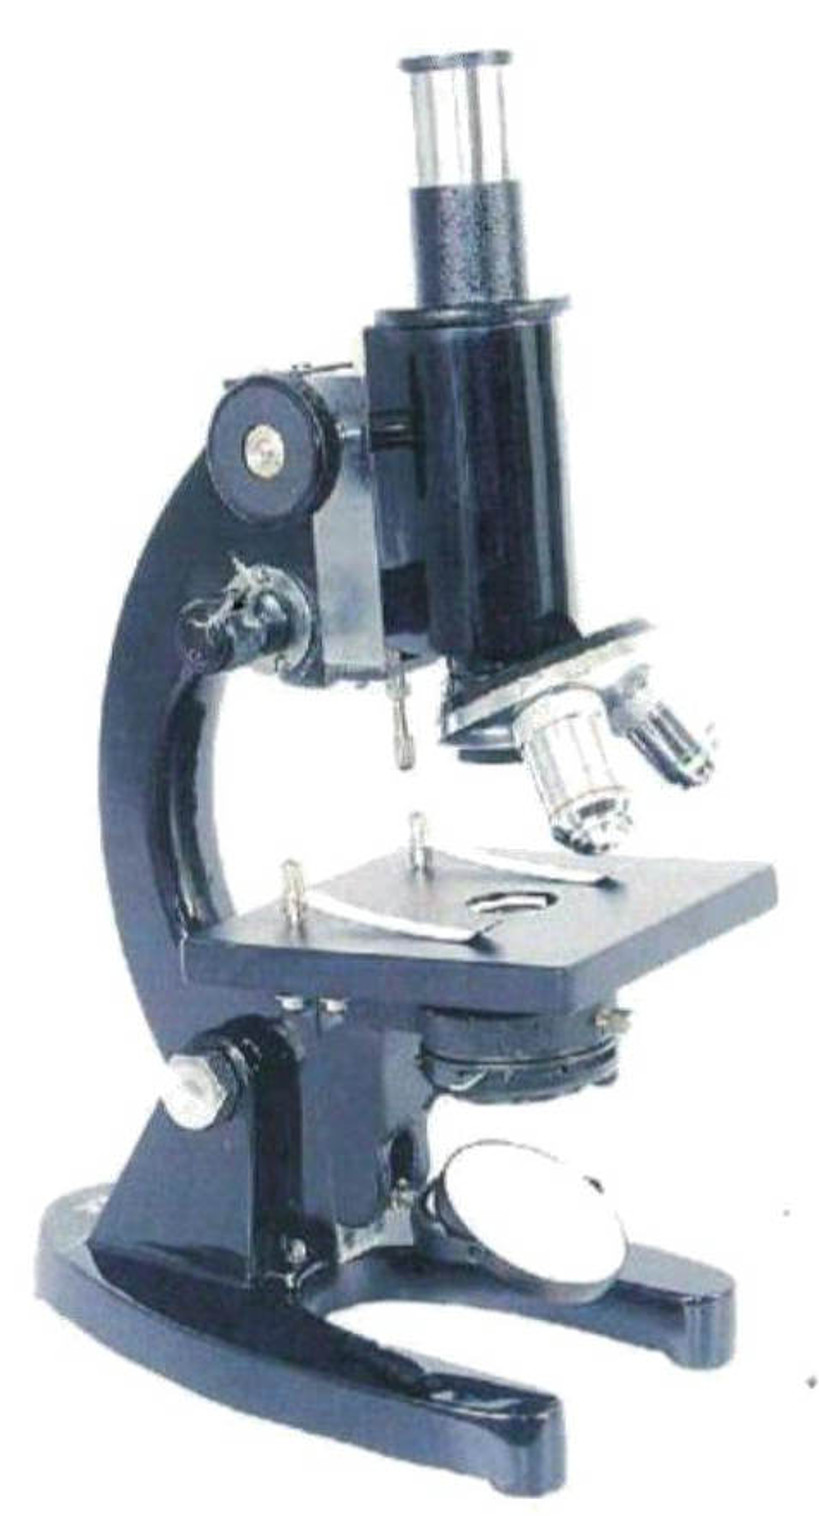
\includegraphics[scale=10]{./compoundMicroscope.jpg}
			\caption*{\textbf{Compound Microscope}}
			\label{compound microscope}
		\end{figure}
		}

		Physical terms:
		\begin{itemize}
			\item{Resolution \par It is the ability to reveal closely adjacent structural details as separate and distinct. The limit of magnification of a microscope is set by its resolving power.}
			\item{Numerical Aperture \par It is the ratio of the diameter of the lens to its focal length. Greater the numerical aperture greater the resolving power.}
			\item{Working Distance \par It is the distance between the objective lens and the slide.}
		\end{itemize}

		\section*{Parts Of The Microscope}

		\subsection*{Support System}
		\begin{enumerate}
			\item{Base \par It supports the microscope on the working table.}
			\item{Pillars \par Two upright pillars project upwards from the base.}
			\item{Handle \par Handle is hinged to the pillars. It supports the magnifying and adjusting systems. It is the handle by which the microscope must be carried. It is curved and the microscope can be tilted at the hinged joint.}
			\item{Body tube \par The eyepiece fits into the top of the body tube. The nose piece with the objective lenses fits into its lower end. It is the part through which the light passes to the eyepiece. It actually conducts the image.}
			\item{Stage \par Fixed stage is the horizontal platform on which the object is placed. It has a central opening through which the illuminating system focuses the light on the object. Mechanical stage has a spring mounted clip to hold the slide or counting chamber in position. It has two screws to move the mounted object from side to side and for ward and backwards.}
			\item {Nose piece \par Fixed nose piece is attached to lower end of body tube. Revolving nose piece carries objective lenses of different magnifying powers.}
		\end{enumerate}

		\subsection*{Adjusting System}
		It consists of the coarse and fine adjustment screws mounted in the handle by a double sided micrometer mechanism.
		\begin{enumerate}
			\item{Coarse adjustment screws \par It consists of rack and pinion which moves the tube rapidly through a large distance when the screw is rotated clockwise or anticlockwise. It is used to obtain an approximate focus of the object.}
			\item{Fine adjustment screws \par Similar to coarse adjustment screw, but several rotations will move the tube through a very small distance. It is used to obtain exact focus of the object.}
		\end{enumerate}

		\subsection*{Illumination System}
		\begin{enumerate}

			\item{Source of illumination \newline
				\par Light source may be internal or external.
				\par Internal source –In modern microscopes, there is an in-built light source with an electrical tungsten lamp, which is placed directly under the stage.
				\par External source – This can be from an electric lamp housed in a lamp box with a window or from the sun. The rays of light are reflected by a mirror towards the object. The mirror is located at the base of the microscope which is plain or concave.}
			\item{Condenser
				\par It focuses the rays of light reflected from the mirror onto the object under observation and helps in resolving the image. It is mounted below the stage of the microscope. Position of the condenser has to be adjusted according to the objective lens used.}
			\item{Iris diaphragm
				\par It is located at the bottom of the condenser. It has a central aperture. The size of the aperture can be altered to regulate the amount of light that passes through the condenser onto the object under observation.}
		\end{enumerate}

		\subsection*{Magnification System}
		\begin{enumerate}

			\item{Eye piece
				\par This is a magnifying lens inserted into the upper end of the body tube. Each eyepiece has two lenses, an eye lens mounted at the top and a field lens at the bottom. It has a magnification power of 5 and 10. It magnifies the primary image to give a virtual image which is observed through the eye piece.}
			\item{Objective lens

				\par Three objective lenses are fitted to the lower end of the body tube in the revolving nose piece. They are the low power, high power and oil immersion objective lenses. The desired objective lens is placed close to object on the stage and it produces a real magnified and inverted primary image. When the oil immersion objective is used, the space between the object and the lens is filled with cedar wood oil which has the same refractive index as that of glass and hence prevents refraction of light.\newline
				\begin{tabular}{c | c | c | c}
					\hline
					Objective & Working Distance & Numerical Aperture &Magnification\\
					\hline
					Low Power & 5 to 15 millm & 0.3 & 10\\
					\hline
					High Power
					&0.5 to 4 millm
					&0.65
					&40/45 \\
					\hline

					%next row
					Oil immersion
					&0.15 to 1.5 millm
					&1.3
					&100 \\

					\hline





				\end{tabular}

				\par
				Adjustments for low power objective
				\begin{itemize}
					\item {Concave mirror is used.}
					\item {Condenser is lowered.}
					\item {Iris diaphragm is slightly opened to decrease the intensity of illumination.}
				\end{itemize}

				\par
				Adjustments for high power objective
				\begin{itemize}
					\item{Concave mirror is used.}

					\item{Condenser is slightly raised.}

					\item{Iris diaphragm is partially opened to increase the intensity of illumination.}
				\end{itemize}

				\par
				Adjustments for oil immersion objective (OPR)
				\begin{itemize}

					\item{Open the Iris diaphragm fully to get maximum intensity of illumination}

					\item{Plane mirror is used.}

					\item{Raise the Condenser.}
				\end{itemize}
				}




			\end{enumerate}

			\section*{Precautions}
			\begin{itemize}
				\item Objectives and eyepiece should be free from dust.
					item The mirror, the position of the condenser, and the aperture of the iris should be checked in order to get proper illumination.
				\item While changing the objective it should be noted that the objective clicks into its proper position.
				\item Do the necessary microscopic adjustments before using each objective.
				\item While focusing, lower the objective close to the slide and focus the object by slowly raising the objective.
				\item Never bring down the objective with the coarse adjustment screw while looking into the microscope.
				\item Examine the slide under low power and high power before examining it under oil immersion objective.
				\item After using oil immersion objective, clean the lens with filter paper and xylol.
			\end{itemize}

			\section*{Questions}
			\begin{enumerate}
				\item Name the oils used for oil immersion objective.
				\item How will you calculate the total magnification power of the microscope for each objective?
				\item Name the other types of microscope.
			\end{enumerate}

			\chapter*{\centering Hemocytometer}
			\begin{tabular}{p{5in} p{1in}}
				\textbf{Exp No:}  & \textbf{Date:}\\
			\end{tabular}

			\addfig{%
				\begin{figure}[h]
					\centering
					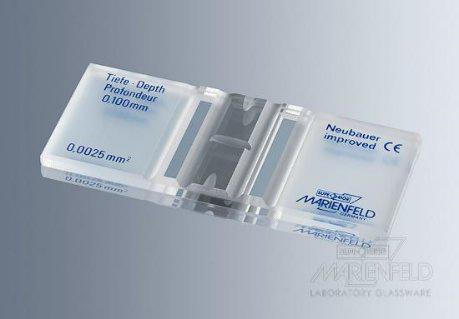
\includegraphics[scale=.5]{./neubar.jpg}
					\caption*{\textbf{Neubauer Chamber}}
					\vspace{1.5cm}
					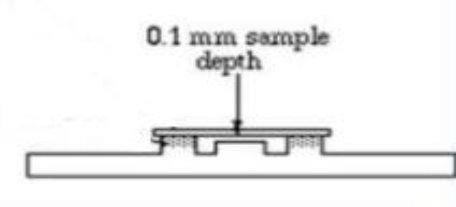
\includegraphics[scale=0.5]{./neubarSide.jpg}
					\caption*{\textbf{Neubauer Chamber - side view}}
					\vspace{2cm}
					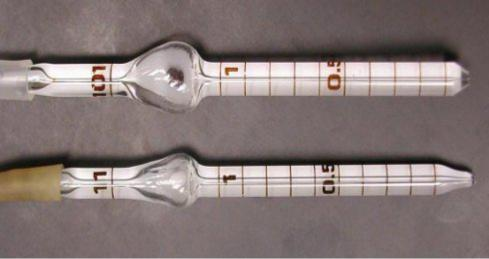
\includegraphics[scale=.5]{./pipette.jpg}
					\caption*{\textbf{RBC \& WBC pipettes}}
					\label{chamber}
				\end{figure}
				}
				\addfig{%
					\begin{figure}[h]
						\centering
						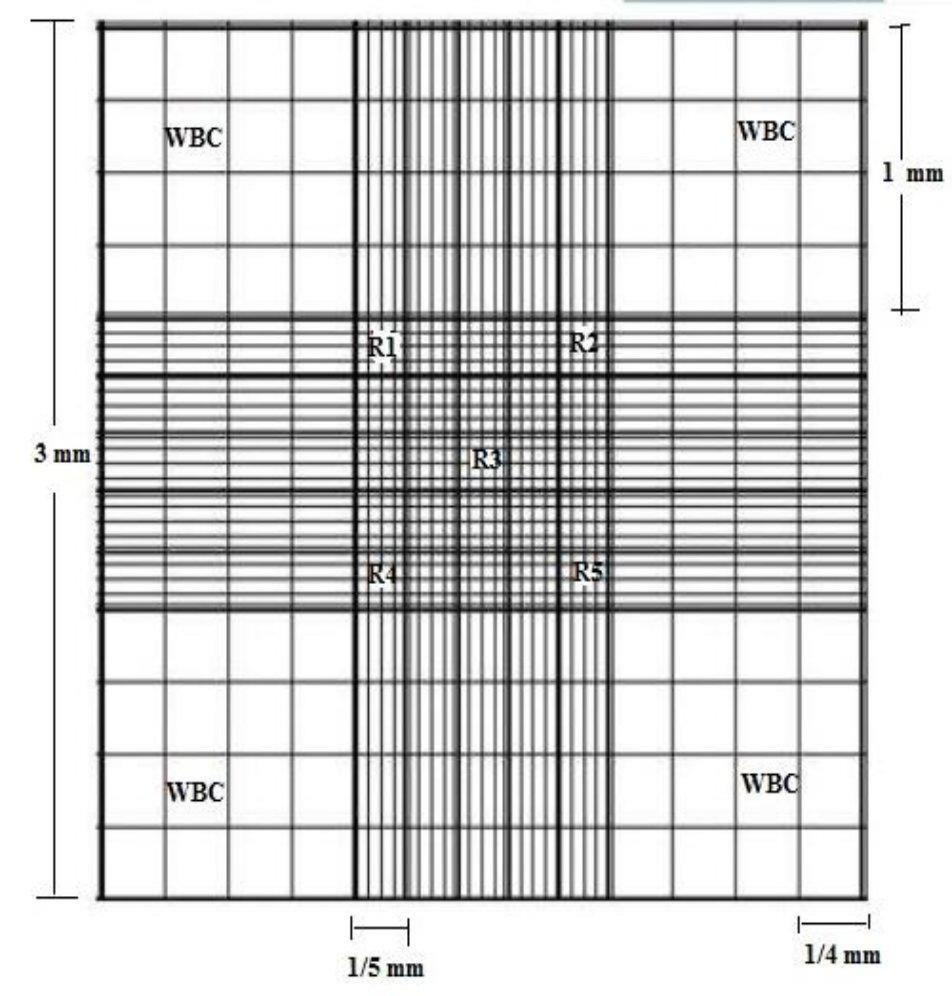
\includegraphics[scale=.5]{./grid.jpg}
						\caption*{\textbf{Neubauer Chamber's Counting Region}}
						\label{grid}
					\end{figure}
					}


					\section*{Introduction}
					The formed elements of blood are counted by Hemocytometry. The apparatus is called as hemocytometer. It consists of diluting pipettes and counting chamber.
					The counting chamber in common use is the improved Neubauer’s counting chamber. This is a thick glass slide divided into two central platforms by a ‘H’ shaped groove. The central platform is slightly lower than the sides. When a cover slip is placed over the central platforms, resting on the side platforms, a space of $\frac{1}{10}$  $mm$ depth will be present between the cover slip and the central platform. This area is used for charging the chamber with the diluted blood for cell counting.
					The central platforms have ruled squares which are used for cell counting. The ruled area is a square measuring 3 $mm$ $\times$ 3 $mm$. This area is divided into 9 large equal squares each having an area of 1 $mm$$^2$. The four large corner squares are used for WBC count. The central square is used for RBC count. All nine squares are used for Absolute eosinophil count.

					\section*{WBC counting squares}
					\begin{itemize}
						\item
							The four large corner squares are used for the WBC count and each has 16 medium squares (16$\times$4=64 medium squares).
						\item {
								Side of each large square is 1 $mm$.}
							\item{
									Area of each large square is 1 $\times$ 1 = 1 $mm$$^{2}$.}
								\item {
										Volume of each large square = area $\times$ depth = 1 $\times$ $\frac{1}{10}$ = $\frac{1}{10}$ $mm^3$.}
								\item{
										Volume of each medium square = $\frac{1}{4}$ $\times$ $\frac{1}{4}$ $\times$ $\frac{1}{10}$ = $\frac{1}{160}$ $mm^3$.}
					\end{itemize}

					\section*{RBC counting squares}
					\begin{itemize}

						\item{The 1$mm^2$ central RBC square is divided into 25 medium sized squares by triple lines. The four corner and central medium sized squares are used for RBC count.}
						\item{Each medium sized square is further divided into 16 small squares.}
						\item{(5 $\times$ 16 = 80 small squares).}
						\item{Side of each medium sized square is $\frac{1}{5}$ $mm$.}
						\item{Area of each medium sized square is $\frac{1}{5}$ $\times$ $\frac{1}{5}$ = $\frac{1}{25}$ $mm^2$.}
						\item{Volume of each medium sized square is $\frac{1}{250}$ $mm^3$.}
						\item{Volume of each smallest square = $\frac{1}{20}$ $\times$ $\frac{1}{20}$ $\times$ $\frac{1}{10}$ = $\frac{1}{4000}$ $mm^3$.}

					\end{itemize}

					\section*{Pipettes}
					The pipettes are used to dilute the blood to a known dilution.
					Two types of pipettes are used – RBC pipette, WBC pipette .
					\par


					Parts of a pipette are:-\newline
					\textbf{The Stem:}
					The long narrow stem has a capillary bore and a well-grounded conical tip. It is divided into 10 equal parts with two numbers etched on it – 0.5 in the middle and 1.0 at the junction of stem and the bulb.\newline
					\textbf{The bulb:}
					The bulb contains a free-rolling bead. The bead helps in identifying the pipette and mixing the diluents with blood in the bulb. Free rolling of the bead in the bulb indicates whether the pipette is dry or not.\newline
					\textbf{Rubber tube and mouthpiece:}
					The narrow rubber tube attached to the bulb, facilitates filling of the pipette by gentle suction. There is a marking just above the bulb. This marking is 11 in WB C pipette and 101 in RBC pipette. The graduations do not indicate absolute or definite amounts in terms of cubic mm .They only indicate relative volumes in relation to each other. The markings indicate relative parts in the pipette\newline

					\subsection*{RBC pipette}
					\begin{itemize}

						\item{Markings are 0.5, 1.0 and 101}
						\item{The capillary bore is narrow}
						\item{Bulb is larger and has a red bead}
						\item{Volume of the bulb is 100 parts}
					\end{itemize}

					\subsection*{WBC pipette:}
					\begin{itemize}
						\item{Markings are 0.5, 1.0 and 11}
						\item{The capillary bore is wider}
						\item{Bulb is smaller and has a white bead}
						\item{Volume of the bulb is 10 parts}
					\end{itemize}


					\subsection*{Finger Prick}
					\begin{itemize}
						\item{Clean the tip of the finger with spirit and allow the area to dry.}
						\item{Prick the tip of finger with the lancet, deep enough to get a good drop of blood.}
						\item{Don’t squeeze the finger pulp after pricking as this leads to the seepage of tissue fluid resulting in dilution of the blood.}
						\item{The prick is usually made on middle or ring finger.}
					\end{itemize}

					\subsection*{Filling The Pipette}
					\begin{itemize}

						\item{Under aseptic precautions prick the finger and wipe away the first drop and allow the flowing blood to form a good sized drop.}
						\item{Hold the pipette horizontally and dip its end into the blood drop. Gently suck blood upto 0.5 or 1.0 mark depending on the dilution required.}

						\item{If the blood overshoots 0.5 or 1.0 mark, remove the excess blood by gently tapping the tip of the pipette on to the palm. Do not use cotton or any absorbent material as it might absorb water content of blood and concentrates blood.}
						\item{Place the tip of the pipette into the diluting fluid and suck upto the 11 mark in case of WBC pipette or 101 mark in case of RBC pipette without any air bubble.}
						\item{Place the pipette horizontally between the palms of both hands with the rubber tube folded parallel to it and roll the pipette for 1-2 minutes, for thorough mixing of blood with the fluid in the bulb.}

					\end{itemize}

					\subsection*{Precautions}
					\begin{itemize}

						\item{The pipette must be dry and free from clotted blood and the bead must roll freely in the bulb.}
						\item{The tip must not press against the finger or be lifted out of the blood drop or else air will enter it.}
						\item{The blood must be diluted immediately, or else it may clot.}
						\item{Always hold the pipette horizontally to avoid leakage of fluid from the pipette while mixing.}

					\end{itemize}


					\subsection*{Focussing The Counting Grid}
					\begin{itemize}

						\item{	Focus the counting grid with low power and then high power objective.}
						\item{	The lines of the squares must be seen clearly.}
					\end{itemize}

					\subsection*{Charging The Chamber}
					\begin{itemize}

						\item{	 Place the coverslip on the central platform of the chamber covering the ruled squares.}
						\item{	 Discard the stem fluid before charging the chamber as it contains only the diluting fluid.}
						\item{	 Form a good drop of diluted blood at the tip of the pipette, by squeezing the rubber tube, while closing its mouthpiece or by gently blowing through the rubber tube.}
						\item{	 Hold the pipette at 45 degree inclination and touch the chamber with the  tip of the pipette between the cover slip and the central platform.}
						\item{	 A thin layer of the fluid spreads under the coverslip on the central  platform by capillary action.}
						\item{	 Avoid overcharging the chamber which is recognized by fluid in the  trenches.}
						\item{	 Wait for 2 minutes for the cells to settle down.}
						\item{	 Focus  the  squares  under  the  desired  objective  and  start  counting.}
					\end{itemize}


					\subsection*{Precautions}
					\begin{itemize}

						\item{	 The chamber and the coverslip should be properly cleaned.}
						\item{	 The contents of the bulb must be thoroughly mixed before charging.}
						\item{	 2-3 drops of fluid must be discarded from the pipette before charging as the stem contains only diluents.}
						\item{	 Air bubbles should not enter the platform of the chamber while charging.}
						\item{	 The chamber should not be overcharged ( gives false low results) or undercharged ( the cells may not be found in peripheral squares).}
					\end{itemize}

					\subsection*{Cell Counting}
					\begin{itemize}

						\item{	 Count the cells in the respective squares.}
						\item{	 Care should be taken not to count the same cells again by following L rule. (Count the cells present inside the square and those on the left and lower lines. Ignore those on the right and upper lines).}
					\end{itemize}

					\subsection*{Questions}

					\begin{enumerate}

						\item{	 What are the other types of cell counting chambers ?}

						\item{	 What are the other cells that can be counted using Neubauer’s chamber?}
						\item{	 Mention the differences between RBC and WBC pipettes.}
					\end{enumerate}

					\chapter*{\centering Estimation Of Total RBC Count}

					\begin{tabular}{p{5in} p{1in}}
						\textbf{Exp No:}  & \textbf{Date:}\\
					\end{tabular}

					\section*{Aim}

					To enumerate the number of  erythrocytes in 1 $mm^3$ of blood.
					\section*{Apparatus Required}
					Microscope, Hemocytometer (RBC diluting pipette and counting chamber), RBC diluting fluid (Hayem’s fluid), spirit, cotton and lancet.

					\section*{Hayem's Fluid - composition}
					\begin{itemize}

						\item{		Sodium chloride - 0.5 g	- Maintains isotonicity}
						\item{		Sodium bisulphate - 2.5 g - Prevents aggregation  of RBCs (Rouleaux formation)}
						\item{		Mercuric perchloride - 0.25 g - Acts  as preservative, antifungal and antibacterial}
						\item{		Distilled water - 100 ml - Acts as solvent}
					\end{itemize}


					\section*{Procedure}

					Make  a  sterile  finger  prick  and  discard  the  first drop  of blood. Draw blood upto  0.5  mark  and  Hayem’s  fluid  upto 101  mark  with  the  pipette. Mix  the contents thoroughly. Discard  the  first  few  drops and then charge  the  Neubauer chamber. Allow  the cells to  settle  for  3-4  minutes.Count the RBCs in the 4 medium sized corner squares and  in the central medium sized square of the RBC counting area (total of 16 x 5 = 80 smallest squares) under high power objective.


					\section*{Calcualtion}
					Number of RBCs in 5 medium sized RBC squares = n\newline\vspace{.4cm}
					Area of 1 medium  sized RBC square =$\frac{1}{5}$ $\times$ $\frac{1}{5}$ = $\frac{1}{25}$ $mm^2$\newline\vspace{.4cm}
					Volume of 1 medium sized RBC square = $\frac{1}{25}$ $\times$ $\frac{1}{10}$ = $\frac{1}{250}$ $mm^3$\newline\vspace{.4cm}
					Volume of 5 medium sized RBC squares = $\frac{1}{250}$ $\times$ 5= $\frac{1}{50}$ $mm^3$\newline\vspace{.4cm}
					Number of cells in  $\frac{1}{50}$ $mm^3$ of diluted blood  = n\newline\vspace{.4cm}
					Number of cells in  1 $mm^3$  of diluted blood = 50 n\newline\vspace{.4cm}
					Dilution factor = 1 : 200\newline\vspace{.4cm}
					Number of cells in 1 $mm^3$ of un diluted blood 	= n $\times$ 50 $\times$ 200  \newline\vspace{.4cm}

					\section*{Result}
					RBC  count in the given  blood sample is $\rule{5cm}{0.1cm}$ cells / $mm^3$
					\section*{Questions}
					\begin{enumerate}

						\item {Name the other diluting fluids used for red  cell count.}
						\item{How will you identify the RBC counting squares?}
						\item{What is the normal RBC count in males and females?}
						\item{Why is the RBC count high in males?}
						\item{Mention the physiological and pathological causes for anemia and polycythemia?}


					\end{enumerate}

					\chapter*{\centering Estimation Of Total WBC Count}

					\begin{tabular}{p{5in} p{1in}}
						\textbf{Exp No:}  & \textbf{Date:}\\
					\end{tabular}
					\section *{Aim}
					To enumerate the number of leucocytes (white blood cells) in 1 $mm^3$ of blood.
					\section*{Apparatus Required}
					Microscope, Hemocytometer, WBC pipette, Turk’s fluid, Spirit, Cotton, Lancet
					\section*{Turk's Fluid Composition}
					\begin{tabular}{l c l}

						1\% Glacial Acetic Acid	&	-&	1.5 ml - Lyses RBCs without affecting WBCs\\
						Gentian Violet&			-&	1.5 ml - Stains nuclei of WBCs\\
						Distilled Water&		-&	100 ml - Acts as solvent\\

					\end{tabular}
					\section*{Procedure}

					Make a sterile finger prick and discard the 1st drop of blood. Draw blood upto 0.5 mark and Turk’s fluid upto 11 mark in the WBC pipette. Mix the contents thoroughly. Discard the first few drops and charge the Neubauer chamber. Allow the cells to settle for 3 to 4 minutes. Count the WBCs in the 4 corner large squares (WBC counting area) under high power objective.

					\section*{Calcualtion}

					Number of cells in 4 WBC squares = n\newline\vspace{.2cm}
					Area of 1 WBC square = 	1$\times$ 1 	= 1 $mm^2$\newline\vspace{.2cm}
					Volume of 1 WBC square	= 1$\times$ $\frac{1}{10}$ = $\frac{1}{10}$ $mm^3$\newline\vspace{.2cm}
					Volume of 4 WBC squares =4$\times$ $\frac{1}{10}$ = $\frac{4}{10}$ $mm^3$\newline\vspace{.2cm}
					Number of cells in $\frac{4}{10}$ $mm^3$ of Diluted blood 	= n \newline\vspace{.2cm}
					Therefore, Number of cells in 1 $mm^3$ of Diluted blood = 	n $\times$ $\frac{10}{4}$\newline\vspace{.2cm}
					Dilution Factor = 1 : 20\newline\vspace{.2cm}
					Therefore, Number of cells in 1 $mm^3$ of Undiluted blood 	= n $\times$ $\frac{10}{4}$ $\times$ 20 =	n $\times$ 50\newline\vspace{.2cm}


					\section *{Result}

					WBC count in the given  blood sample is $\rule{5cm}{0.1cm}$ cells / $mm^3$

					\section*{Questions}


					\begin{enumerate}

						\item{What is the normal RBC : WBC ratio ?}
						\item{ In which condition is RBC pipette used for counting WBCs ?}
						\item{ Why is blood diluted only 20 times in WBC counting?}
						\item{ Mention the physiological and pathological causes of high and low WBC count.}
						\item{ What is Leucocytosis ?}
						\item{ What is Leukemia?}
					\end{enumerate}

					\chapter*{\centering Absolute Eosinophil Count}

					\begin{tabular}{p{5in} p{1in}}
						\textbf{Exp No:}  & \textbf{Date:}\\
					\end{tabular}

					\section*{Aim}

					To determine the number of eosinophils per cu mm of blood
					\section*{Apparatus Required}
					Microscope, Hemocytometer, Dunger’s fluid, spirit, cotton and lancet.
					\section*{Dunger's Fluid Composition}
					1\% of solution of eosin in water (5$ml$)- Eosin stains the eosinophilic granules.\newline
					Acetone (5$ml$) - Acetone lyses the cell membrane of all other cells.\newline
					Distilled water (90$ml$) - Distilled water to make up to 100$ml$.Acts as solvent.\newline
					\section*{Procedure}
					Make a sterile finger prick and discard the first drop of blood. Draw blood upto 1 and the Dunger’s fluid upto mark 11 in a WBC pipette. Mix the contents thoroughly. Cover the pipette with a petri dish lined by moistened filter paper. Wait for 15 minutes. Discard the first few drops and charge the Neubauer chamber. The eosinophils are identified by the pinkish orange stained coarse granules in the cytoplasm. Count the Eosinophils in all the 9 large squares of the Neubauer chamber. Count within 30 minutes of charging .
					\section*{Calcualtion}
					Number of cells counted in 9 large squares				=	n\newline\vspace{.2cm}
					Area of 1 large square				=	1 $\times$ 1		=	1$mm^2$	\newline\vspace{.2cm}
					Volume of 1 large square				=	1 $\times$ $\frac{1}{10}$	=	$\frac{1}{10}$ $mm^3$\newline\vspace{.2cm}
					Volume of 9 large square				=	9 $\times$ $\frac{1}{10}$	=	$\frac{9}{10}$ $mm^3$\newline\vspace{.2cm}
					Number of cells in $\frac{9}{10}$ $mm^3$ of diluted blood				=	n\newline\vspace{.2cm}
					Number of cells in 1 $mm^3$ of diluted blood				=	n $\times$ $\frac{10}{9}$\newline\vspace{.2cm}
					Dilution factor								=	1:10\newline\vspace{.2cm}
					Therefore, number of cells in 1 $mm^3$ of undiluted blood		=	n$\times$$\frac{10}{9}$$\times$10
					=	n$\times$$\frac{100}{9}$
					\section*{Result}

					Abosolute Eosinophil count in the given  blood sample is $\rule{5cm}{0.1cm}$ cells / $mm^3$

					\section*{Questions}
					\begin{enumerate}

						\item{What is the normal value of Absolute Eosinophil Count ?}
						\item{What is the difference between the Differential Count and the Absolute Eosinophil Count ?}
						\item{What are the other diluting fluids used for Absolute Eosinophil Count?}
						\item{What are the contents of eosinophilic granules ?}
						\item{What are the functions of eosinophils?}
						\item{What are eosinopenia and eosinophilia?}
					\end{enumerate}

					\chapter*{\centering Diffrential Count}
					\begin{tabular}{p{5in} p{1in}}
						\textbf{Exp No:}  & \textbf{Date:}\\
					\end{tabular}

					\section*{Aim}
					To determine the differential count of White Blood Cells.
					\section*{Apparatus Required}
					Grease free and dry glass slides, Leishman’s stain, distilled water, lancet, spirit, cotton.	
					\section*{Leishman's Stain Composition \& Functions}
					Methylene blue (basic) 	     -	Stains acidic granules in cytoplasm especially 						granules of basophils and Nuclei of leucocytes.\newline
					Eosin (acidic) 		     -	Stains cytoplasm, basic granules in 							cytoplasm, Hemoglobin of RBCs.\newline
					Acetone free methyl alcohol - 	Fixes the cells (Acetone free methyl alcohol 						is used as acetone is a lipid solvent that 		lyses cell membrane).\newline 

					\section*{Procedure}

	\addfig{%
		\begin{figure}[h]
			\centering
			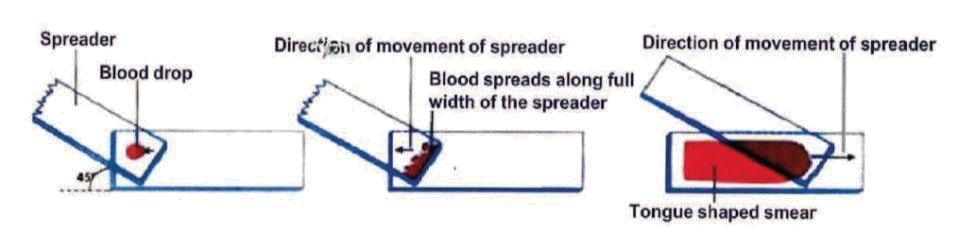
\includegraphics[scale=.50]{./smear1.jpg}
			\label{smear1}
			\vspace{3cm}
			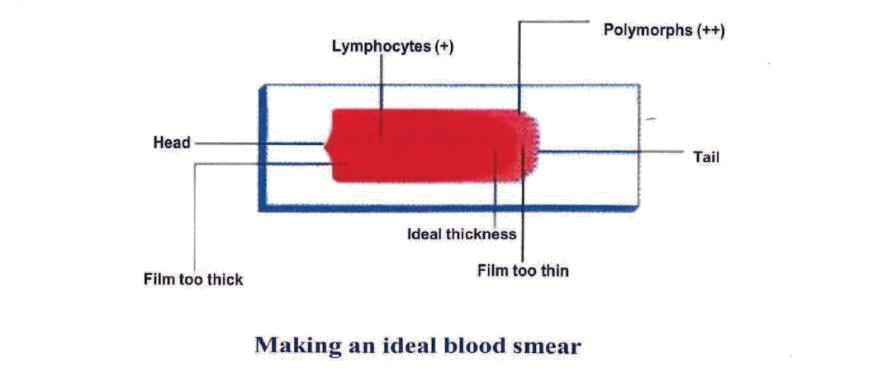
\includegraphics[scale=.50]{./smear2.jpg}
			\label{smear2}
			\vspace{1cm}
			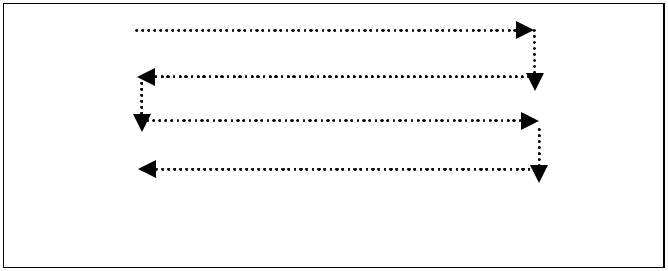
\includegraphics[scale=.50]{./smear3.jpg}
			\label{smear3}
		\end{figure}
		}
					Under aseptic precautions, prick the finger. Discard the first drop of blood. Place the slide on the table and support with left hand. Place the blood drop on the right end, one cm away from the edge. Place the spreader slide just infront of the blood drop. Draw the spreader slide backwards to touch the drop. The blood spreads across the edge of the spreader. Draw the spreader slide forward at an angle of 45$^{\circ}$ with a smooth, fast and firm movement to make a thin tongue shaped blood smear. Too thick, thin or a patchy smear is to be avoided. Air dry the smear quickly.

					Place the glass slide with the smear on a tray and add Leishman’s stain, drop by drop till the entire smear is covered with the stain. Count the number of drops added. Note the time and wait for 2 minutes (Fixation time). After 2 minutes, add double the quantity of distilled water over the film using a dropper. See to that the distilled water uniformly covers the entire surface of the slide and dilutes the stain homogenously. Gently blow the stain and the distilled water from one end of the slide to the other for uniform mixing. Wait for about 8-10 minutes for the smear to take up the stain uniformly (Staining time).
					Flush the slide under a gentle stream of tap water to remove the excess stain. Dry the slide. Scan the film under low \& high power objective. Make necessary microscopic adjustments for oil immersion objective (100X). Add a drop of cedar wood oil over the smear at the junction between the body and the tail, as the smear will be of one cell thickness with uniform staining here. Cedar wood oil has the same refractive index as that of glass and minimizes refraction. Examine in a zig-zag manner as shown in the figure.

					Draw a table with 100 squares to count 100 WBCs and enter the type of cell as identified while examining the film.

	\addfig{%
		\begin{figure}[h]
			\centering
			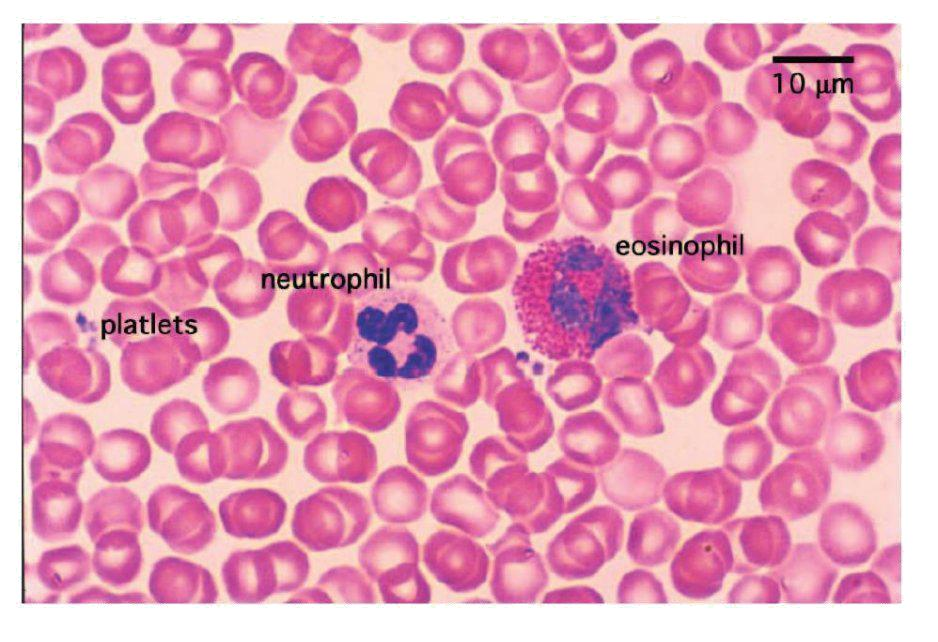
\includegraphics[scale=13]{./dc1.jpg}
			\label{dc1}
			\vspace{3cm}
			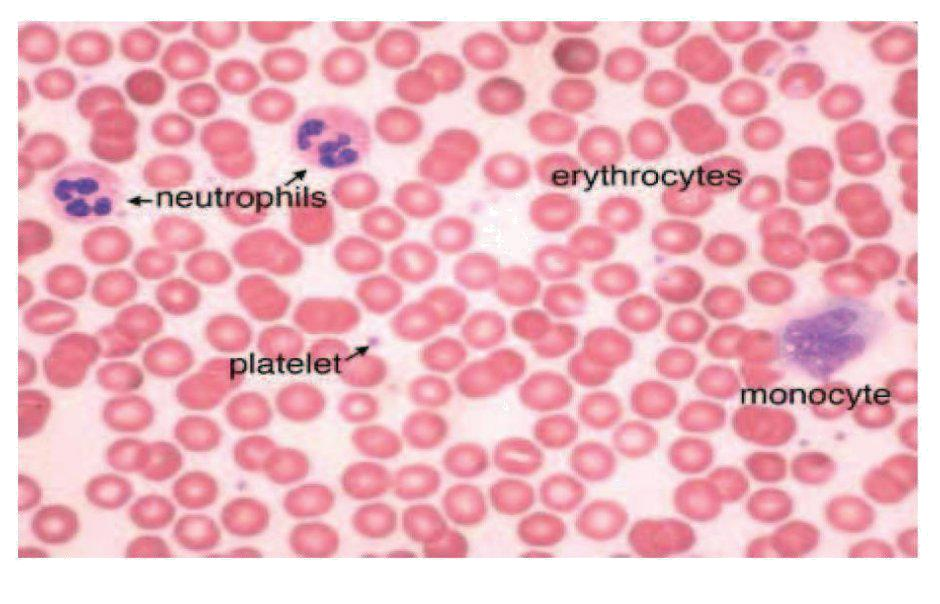
\includegraphics[scale=13]{./dc2.jpg}
			\label{dc2}
		\end{figure}
		}
					Under aseptic precautions, prick the finger. Discard the first drop of blood. Place the slide on the table and support with left hand. Place the blood drop on the right end, one cm away from the edge. Place the spreader slide just infront of the blood drop. Draw the spreader slide backwards to touch the drop. The blood spreads across the edge of the spreader. Draw the spreader slide forward at an angle of 45$^{\circ}$ with a smooth, fast and firm movement to make a thin tongue shaped blood smear. Too thick, thin or a patchy smear is to be avoided. Air dry the smear quickly.

					\section*{Result}
					The differential count of WBCs in the blood sample is as follows.\newline
					Neutrophil = $\rule{5cm}{0.1cm}$ \%\newline
					Eosinophil = $\rule{5cm}{0.1cm}$ \%\newline
					Basophil = $\rule{5cm}{0.1cm}$ \%\newline
					Lymphocyte = $\rule{5cm}{0.1cm}$ \%\newline
					Monocyte =$\rule{5cm}{0.1cm}$ \%\newline

					\section*{Questions}
					\begin{enumerate}
						\item{Draw the different WBCs using appropriate colours.}
						\item{What other cells can you visualize in the smear?}
						\item{Enumerate the criteria of a good blood smear.}
						\item{Can tap water be used for dilution? why?}
						\item{Mention the functions of various types of WBCs and their abnormalities in count.}
						\item{Mention the clinical importance of peripheral blood smear.}
					\end{enumerate}


					\section*{Identifcation Of The Cells}
					A leukocyte is identified by its size, nucleus, cytoplasm and granules.

					\begin{tabularx}{\textwidth}{*{5}{m{.2\textwidth}|X|}}
%{|c|c|X|X|c|}
						\hline
						\textbf{Cell type}&
						\textbf{Size}&
						\textbf{Nucleus}&
						\textbf{Cytoplasm}&
						\textbf{Normal Values}\\

						\hline

						Neutrophil&
						10 – 14 ${\mu}m$&
						2-5 lobes connected by narrow strands of chromatin&
						Fine violet-pink granules&
						60-70\%\\

						\hline
						Eosinophil&
						10 - 15 ${\mu}m$&
						Often bi-lobed connected by thick strands of chromatin (spectacle shaped nucleus)&
						Coarse brick-red to orange granules&
						2-8\%\\
						\hline	

						Basophil&
						10 - 15 ${\mu}m$&
						Irregularly shaped (S shaped) nucleus masked by the granules&
						Very coarse deep purple granules&
						0-1\%\\
						\hline

						Small lymphocyte&
						7-9 ${\mu}m$&
						Single, round, almost fills the cell Thin cresent of clear, light blue cytoplasm. &
						No visible granules.&
						\multirow{2}{*}{20-30\%}\\
						\cline{1-4}

						Large lymphocyte&
						10 - 15 ${\mu}m$&
						Single, round, almost fills the cell.  May be central or eccentric.&
						Large cresent of clear, light blue cytoplasm. No visible granules.&
						\\
						\hline

						Monocyte&
						12 - 20 ${\mu}m$&
						Horse-shoe shaped nucleus Indented&
						Abundant, muddy blue in appearance. No visible granules.&
						1-5\%\\
						\hline
					\end{tabularx}	





					\chapter*{\centering Hemoglobin Estimation}
					\begin{tabular}{p{5in} p{1in}}
						\textbf{Exp No:}  & \textbf{Date:}\\
					\end{tabular}

					\section*{Aim}
					\section*{Apparatus Required}
					\section*{Turk's Fluid Composition}
					\section*{Procedure}
					\section*{Calcualtion}
					\section*{Result}
					\section*{Questions}

					\chapter*{\centering Blood Grouping \& Typing}
					\begin{tabular}{p{5in} p{1in}}
						\textbf{Exp No:}  & \textbf{Date:}\\
					\end{tabular}

					\section*{Aim}
					\section*{Apparatus Required}
					\section*{Turk's Fluid Composition}
					\section*{Procedure}
					\section*{Calcualtion}
					\section*{Result}
					\section*{Questions}

					\chapter*{\centering Estimation Of Erythrocyte Sedimentation Rate}
					\begin{tabular}{p{5in} p{1in}}
						\textbf{Exp No:}  & \textbf{Date:}\\
					\end{tabular}
					\section*{Aim}
					\section*{Apparatus Required}
					\section*{Turk's Fluid Composition}
					\section*{Procedure}
					\section*{Calcualtion}
					\section*{Result}
					\section*{Questions}


					\chapter*{\centering Packed Cell Volume}
					\begin{tabular}{p{5in} p{1in}}
						\textbf{Exp No:}  & \textbf{Date:}\\
					\end{tabular}
					\section*{Aim}
					\section*{Apparatus Required}
					\section*{Turk's Fluid Composition}
					\section*{Procedure}
					\section*{Calcualtion}
					\section*{Result}
					\section*{Questions}


					\chapter*{\centering Osmotic Fragility}
					\begin{tabular}{p{5in} p{1in}}
						\textbf{Exp No:}  & \textbf{Date:}\\
					\end{tabular}

					\section*{Aim}
					\section*{Apparatus Required}
					\section*{Turk's Fluid Composition}
					\section*{Procedure}
					\section*{Calcualtion}
					\section*{Result}
					\section*{Questions}

					\chapter*{\centering Specific Gravity}

					\begin{tabular}{p{5in} p{1in}}
						\textbf{Exp No:}  & \textbf{Date:}\\
					\end{tabular}

					\section*{Aim}


					\section*{Apparatus Required}
					\section*{Turk's Fluid Composition}
					\section*{Procedure}
					\section*{Calcualtion}
					\section*{Result}
					\section*{Questions}


					\part{Clinical Physiology}


				\end{document}
